
\chapter{Análise bibliográfica sobre simulações e experimentos voltados para a influência de opniões, por Gabriel Ligoski\label{chap:bibliometria:gabrielligoski}}

\section{Planejamento do estudo}
O interesse pelo tema surgiu das recentes problemáticas envolvendo a manipulação de opnião pública, a internet como meio propagador e as consequências destes problemas.
Algo muito comum por exemplo são empresas pagarem para pessoas publicarem críticas positivas sobre seus produtos para assim influenciar pessoas a se tornarem consumidores e depois postarem positivamente sobre este produto, como demonstrado neste vídeo \cite{linus_tech_tips_its_2022}, pessoas chegam a enganarem seus sentidos para fazer parte de um grupo de opniões.
\cite{anderson_development_2014} fizeram um modelo de simulação baseado em liderança de opinião sobre enfermeiras, para agilizar o processo de aprendizagem e melhorar os resultados do hospital. A opinião de enfermeiras com autoridade, ou seja mais capacitadas, trazia segurança e influenciava nas decisões e opniões de outras enfermeiras. Neste estudo a influência foi utilizado de forma positiva.

No caso do meu trabalho, as perguntas que o nortearam foram:
\begin{itemize}
    \item É possível prever a prevalência de opniões baseado na sua popularidade?
    \item Como pode haver harmonia entre opniões divergentes?
    \item Como grupos de agentes com ideias semelhantes se formam e evoluem?
    \item Porque fragmentos de opniões tendem a desaparecer?
\end{itemize}

\section{Coleta de dados}
A coleta de dados feita usando a Scopus no dia 06 de dezembro de 2022, acessado por meio do
Portal de Periódicos da CAPES.

\subsection{Query da busca}
Foi utilizada a query: 
\begin{verbatim}
TITLE-ABS-KEY ( ( "experiment" OR "simulation" OR "multi-agent" ) AND ( "opinion seeking" OR "word of mouth" OR "opinion leader" OR "user influence" ) ) AND PUBYEAR > 2000 AND PUBYEAR < 2023 AND ( LIMIT-TO ( LANGUAGE , "English" ) )
\end{verbatim}
Fora pesquisado ao menos um entre experimento, simulação e multi-agente e ao menos um entre busca de opinião, boca a boca, lider de opinião e influência de usuário. Aplicados no título, abstract, author e keywords. Filtrando para publicações a partir do ano 2000 e em inglês.

\subsection{Registros recuperados}
Foram obtidos 1,621 documentos que encontram-se em \url{https://github.com/gabrielligoski/bibliographic-analysis-of-opinion-influence/}.
Para obter estes documentos utilizei a opção de exportar como csv todos os documentos da pesquisa e selecionei todos os campos.

\section{Análise dos dados}
\subsection{Filtros}
Foi aplicado os filtros de data e linguagem, filtrando todos os artigos dentro do período de 2000 a 2023 e em inglês.

\subsection{Análise descritiva do dataset}

As informações mais gerais sobre o dataset são as seguintes:
\begin{description}
    \item [Crescimento anual] Em média cresceu 20.21\% ao ano com ano de maior crescimento e publicações 2021.
    \item [Média de citação anual] Em média foram 14 citações, com o ano de 2003 distoante com 35 citações médias por artigo publicado.\footnote{Note que neste ano houveram apenas 4 documentos obtidos, por isso provavelmente um deles causou essa discrepancia.}.
    \item [Fonte mais relevante] A fonte com maior quantidade de artigos foi \begin{verbatim}
LECTURE NOTES IN COMPUTER SCIENCE (INCLUDING SUBSERIES LECTURE NOTES IN ARTIFICIAL INTELLIGENCE AND LECTURE NOTES IN BIOINFORMATICS)
\end{verbatim}
    \item [Campo de pesquisa mais relevante] Computadores em comportamento humano, isso é um reflexo de como as novas tecnologias principalmente redes sociais veem impactando o comportamento humano.
    \item [Autores mais relevantes] Liu Y e Wang X lideram o quadro de documentos publicados com 22 cada.
    \item [Países lideres em citação] USA lidera com 18311 citações, logo em seguida vem China com 3442, Koreia com 1994, Alemanha com 1871 e Reino Unido com 1498. \footnote{O número de citações dos USA provavelmente se deve ao filtro de linguagem imposto.}.
\end{description}

\subsection{Evolução da Produção Científica}

\begin{figure}
    \centering
    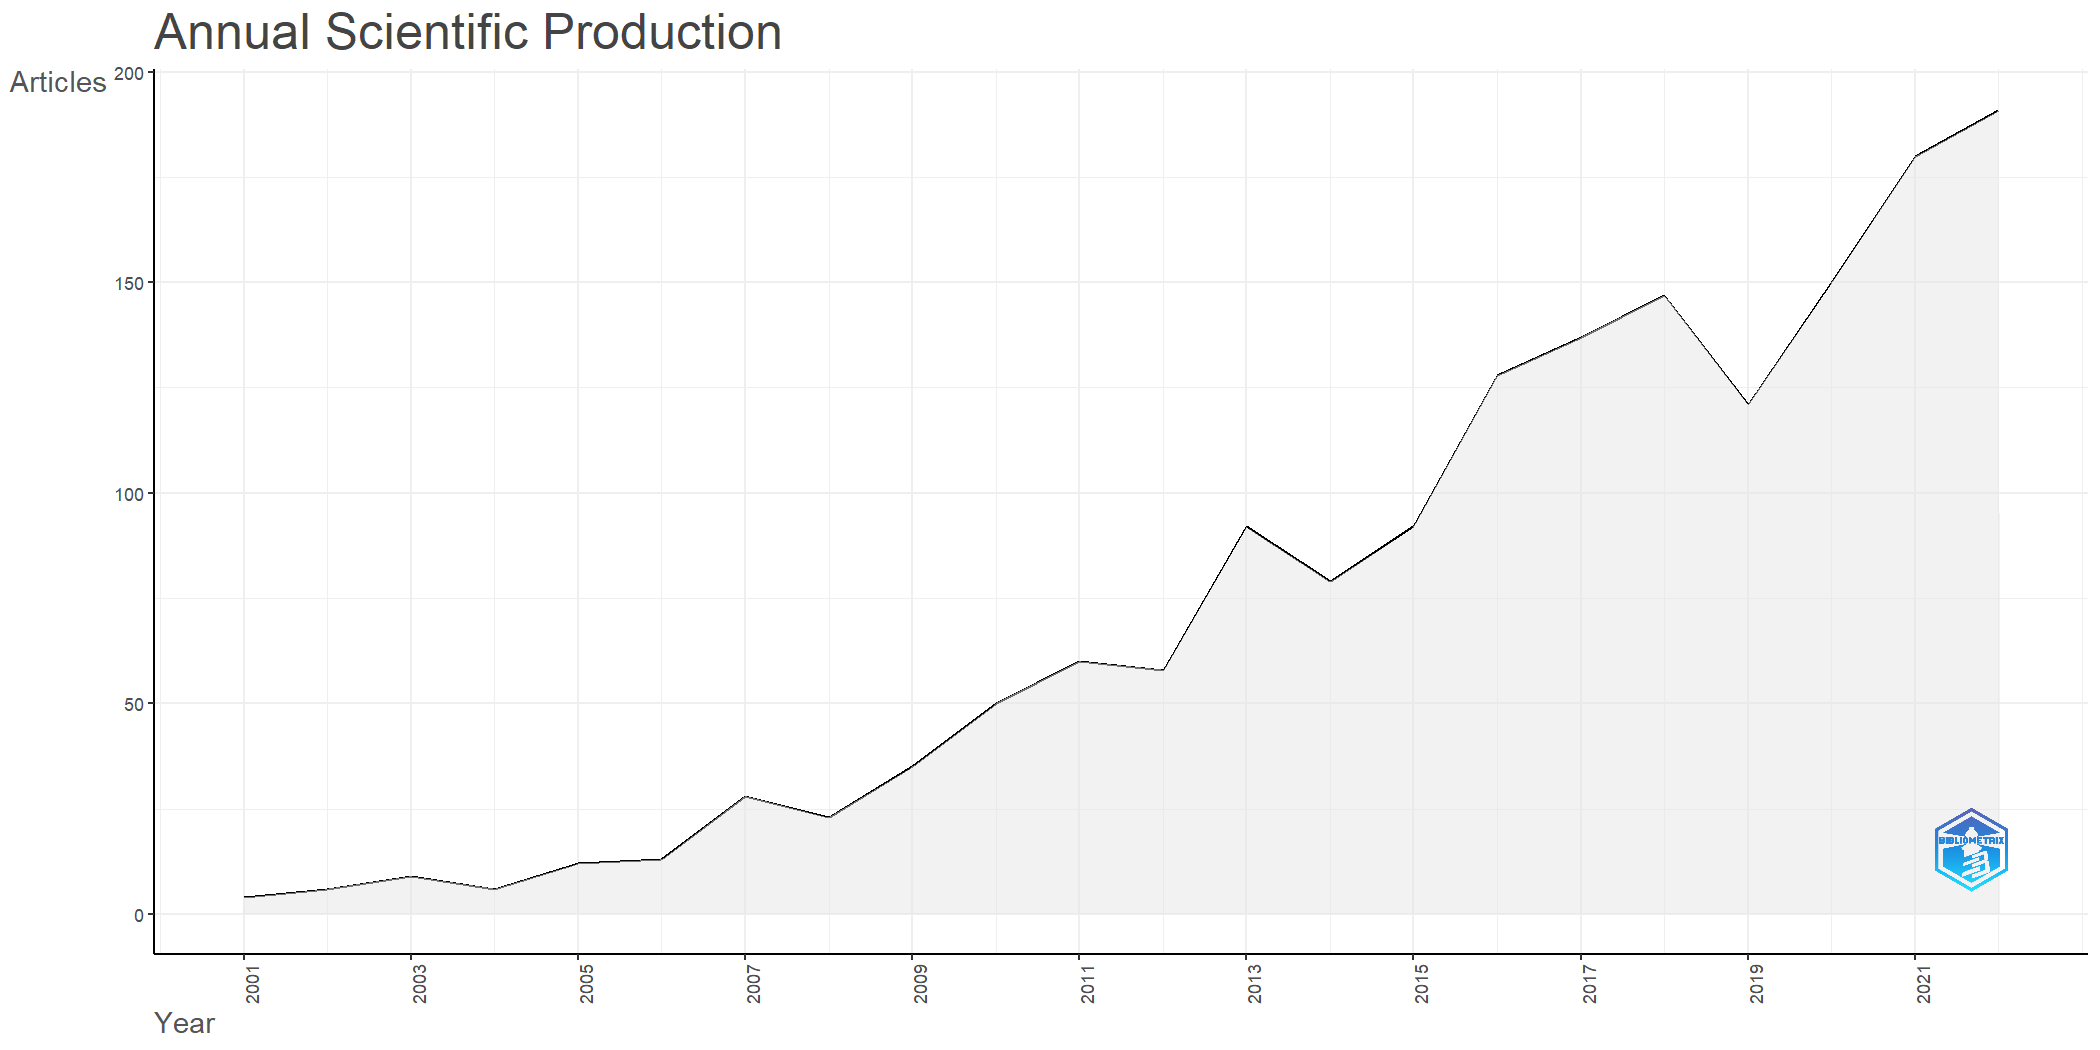
\includegraphics[width=1\textwidth]{exploratory-data-analysis/gabrielligoski/PesqBibliogr/ColorPatches/AnnualScientificProduction-2022-12-06.png}
    \caption{Evolução da produção científica no dataset}
    \label{fig:evol:anual:gabrielligoski}
\end{figure}

A produção de Conteúdo científico deste tema vem crescido a uma taxa acelerada indicando uma possível tendência de popularidade para os próximos anos e que é um tema pertinente principalmente se tratando de temas muito discutidos como o impacto/influência de redes socias para disciminação de opiniões, com uso de ferramentas como twitter.

\subsection{Evolução da Produção Científica}

\begin{figure}
    \centering
    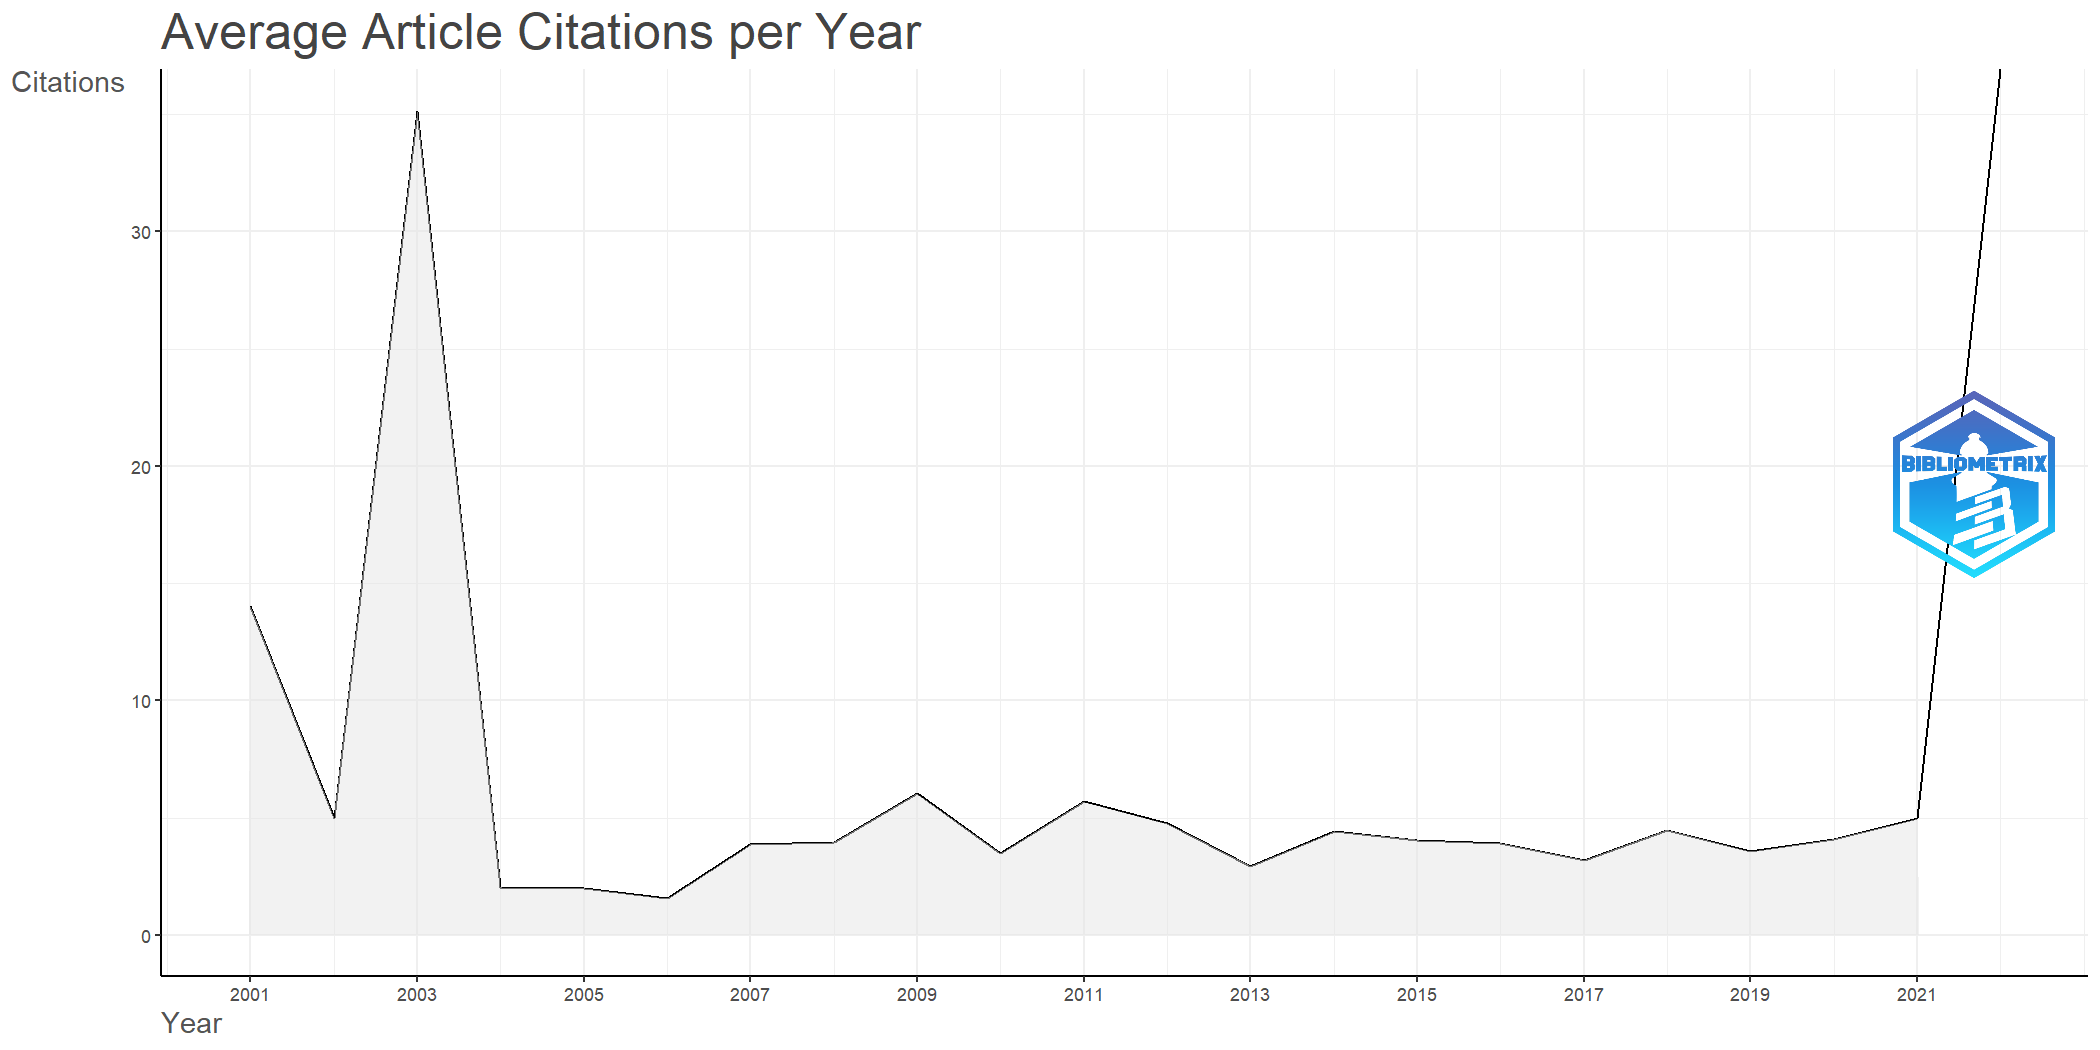
\includegraphics[width=1\textwidth]{exploratory-data-analysis/gabrielligoski/PesqBibliogr/ColorPatches/AverageArticleCitationPerYear-2022-12-06.png}
    \caption{Média de citações anuais no dataset}
    \label{fig:cit:anual:gabrielligoski}
\end{figure}

O gráfico tem um pico em 2003 por se tratar de um baixo número de artigos que foram muito citados, porém é interessante ver que mesmo com um crescente número de documentos cientificos o número se manteve constante após 2003 indicando um crescimento orgânico do interesse pelo tema.


\subsection{Relação palavra-chave a país}

\begin{figure}
    \centering
    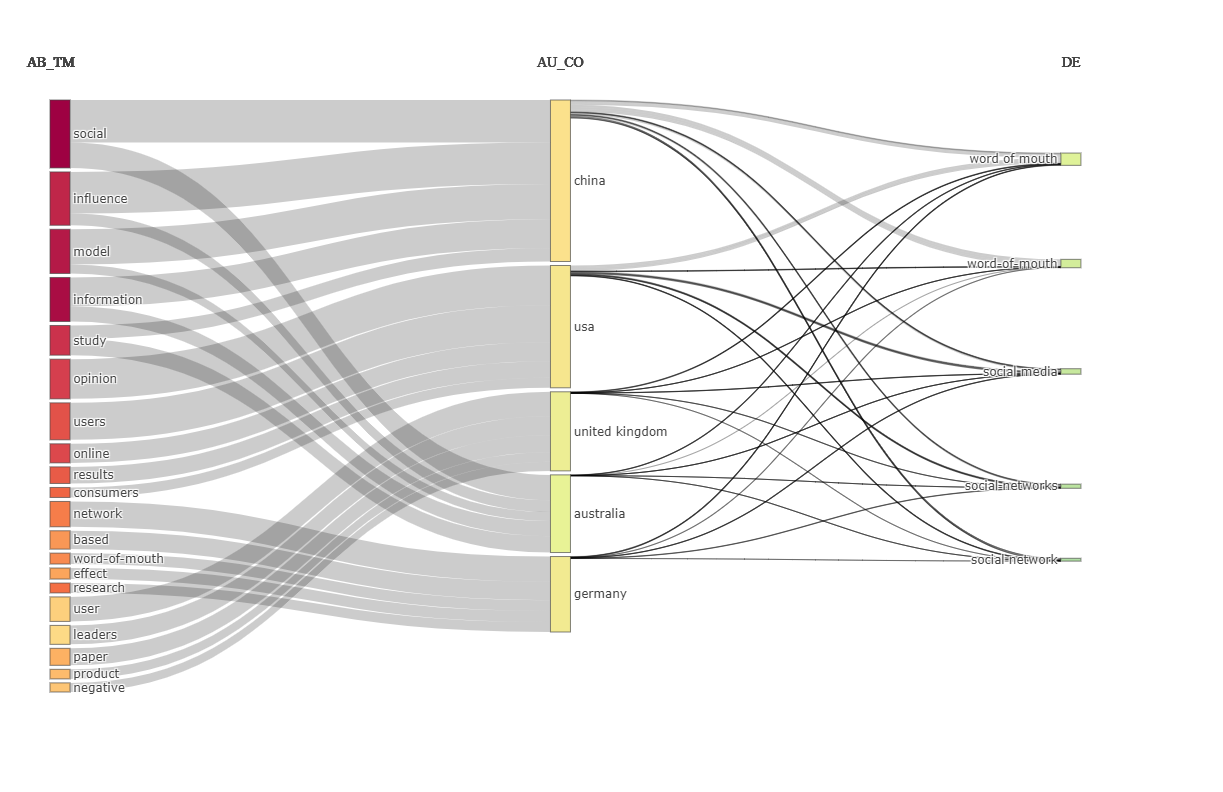
\includegraphics[width=1\textwidth]{exploratory-data-analysis/gabrielligoski/PesqBibliogr/ColorPatches/threeFieldPlot.png}
    \caption{Análise do interesse por país e palavra-chave}
    \label{fig:cit:anual:gabrielligoski}
\end{figure}

Analisando o gráfico podemos ver uma tendência do interesse de cada país por algum campo específico, os USA e Reino Unido parecem buscar mais o interesse econômico destes estudos com foco em opinião, usuários, resultados e consumidores. Enquanto a China, Australia e Alemanha tem um interesse maior em efeitos sociais com foco em social, influência e informação.


\subsection{Relevância de temas}

\begin{figure}
    \centering
    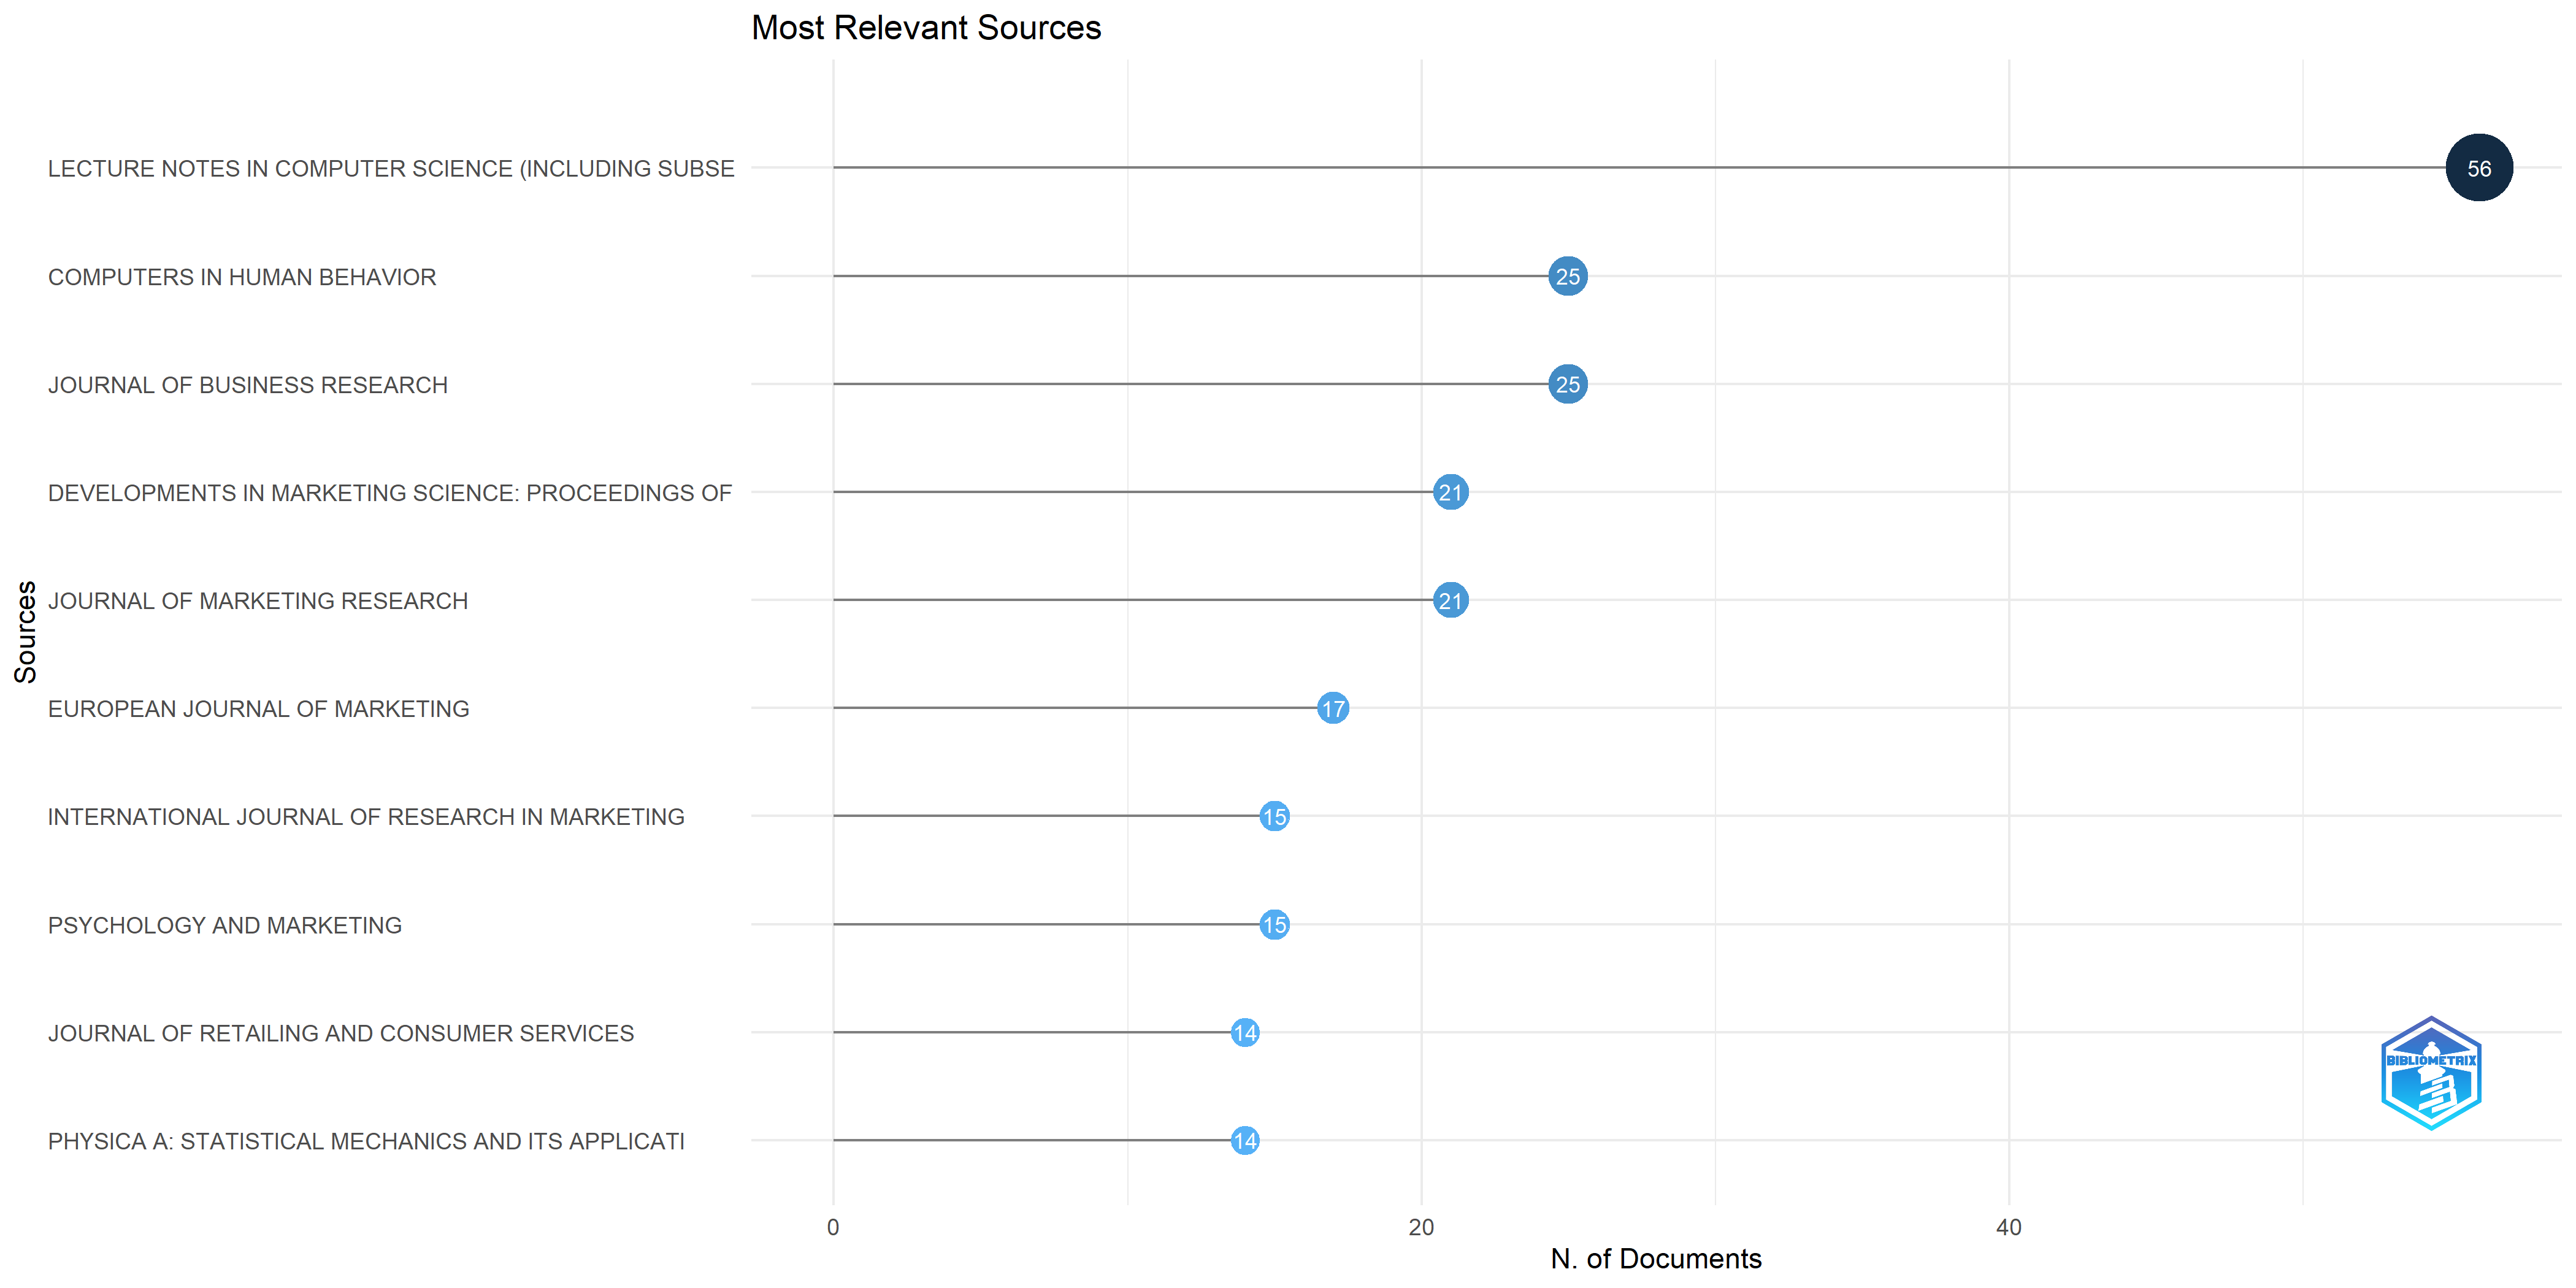
\includegraphics[width=1\textwidth]{exploratory-data-analysis/gabrielligoski/PesqBibliogr/ColorPatches/MostRelevantSources-2022-12-06.png}
    \caption{Relevância de temas pelo abstract}
    \label{fig:cit:anual:gabrielligoski}
\end{figure}

Analisando o gráfico podemos ver que boa parte se deve ao quesito de simulação e modelo, pois a maioria vem de ciência da computação.

\subsection{Autores}

\begin{center}
\begin{tabular}{||c c ||} 
\hline
 Author & Artigos\\ [0.5ex] 
 \hline\hline
LIU Y	& 22\\ \hline
WANG X	& 22\\ \hline
ZHANG Y	& 19\\ \hline
LI Y	& 18\\ \hline
WANG Y	& 15\\ \hline
WANG H	& 14\\ \hline
LI H	& 13\\ \hline
WANG J	& 13\\ \hline
ZHANG J	& 13\\ \hline
CHEN Y	& 12\\ \hline
\end{tabular}
\end{center}

Vendo a tabela com os 10 autores com maior número de artigos podemos ver um grande interesse e investimento  por parte dos chineses.

\subsection{Disputa demográfica}

\begin{center}
\begin{tabular}{||c c c ||} 
\hline
 Country & Year & Articles\\ [0.5ex] 
 \hline\hline
CHINA	& 2022	& 1590\\ \hline
CHINA	& 2021	& 1391\\ \hline
USA	& 2022	& 1205\\ \hline
CHINA	& 2020	& 1181\\ \hline
USA	& 2021	& 1054\\ \hline
CHINA	& 2019	& 1022\\ \hline
USA	& 2020	& 949\\ \hline
CHINA	& 2018	& 891\\ \hline
USA	& 2019	& 846\\ \hline
USA	& 2018	& 734\\ \hline
\end{tabular}
\end{center}

Ordenando pelo número de artigos podemos ver que a China e os USA vem liderando os investimentos no campo, com o interesse de políticos no aspecto da opinião pública é compreensível que haja um bom investimento por países com grande interesse no controle mundial das opiniões e cultura.


\begin{center}
\begin{tabular}{||c c c ||} 
\hline
From &	To &	Frequency\\ [0.5ex] 
 \hline\hline
CHINA	& USA	& 74\\ \hline
CHINA	HONG & KONG	& 23\\ \hline
CHINA	& AUSTRALIA	& 20\\ \hline
USA	& KOREA	& 19\\ \hline
USA	& CANADA	& 17\\ \hline
USA	UNITED & KINGDOM	& 13\\ \hline
CHINA	UNITED & KINGDOM	& 8\\ \hline
USA	HONG & KONG	& 8\\ \hline
USA	& NETHERLANDS	& 8\\ \hline
GERMANY	& DENMARK	& 7\\ \hline\hline
 Country & Year & Articles\\ \hline
\end{tabular}
\end{center}

Ordenando pela frequência vemos que China colabora bastante com os USA, porém isso não é reciproco, possivelmente por conta da linguagem dos documentos que não obteve documentos chineses.

\section{Análise dos documentos}
\subsection{Previsibilidade}
Em \cite{aral_creating_2011} é estudado a influência de empresas em contágio social, buscando a criação de um "boca a boca" eficiente, que efetivamente é criar uma opinião sobre uma marca ou produto. Neste estudo é possível prever até certo ponto o sucesso de uma "opinião" criada por uma marca com base no recurso utilizado para viraliza-la.

\subsection{Ideias contrárias}
Em \cite{bail_exposure_2018} criam-se robôs para postar no twitter opiniões divergentes nos USA, um para democratas e outro para republicanos, o comportamento dos robôs era responder automaticamente posts de seus pares com ideias  contrárias, ao final do estudo pode-se notar que o robô conseguiu mudar um pouco da opinião de seus seguidores acumulados. Criando de certa forma uma pequena tendencia de harmonia entre ideias opostas.

\subsection{Fragmentos e minorias}
Em \cite{chen_online_2011} foi estudado a influência da opinião de outros consumidores pelo boca a boca e avaliações do produto, buscando o impacto na opinião de outros consumidores, notaram que as avaliações positivas impactaram o número de vendas porém as avaliações negativas tiveram um impacto negligente. Possivelmente a vontade das pessoas de fazer parte da opinião de um grupo grande impacta nestas decisões, assim as pessoas avaliam positivamente os produtos pelo que lhes foi dito. Assim como acontece no vídeo \cite{linus_tech_tips_its_2022}, dessa forma fragmentos tendem a desaparecer.